%-----------------------------Modelo Esturctural de Profesores--------------------------%
\section{Modelo Estructural de Profesores}
En la figura \ref{fig:infoProfesores} se puede observar la información que el \refElem{Calmecac} utilizará de acuerdo a los servicios web proporcionados por el \refElem{SIEE}.%Verificar

\begin{figure}[hbtp!]
	\begin{center}
	\fbox{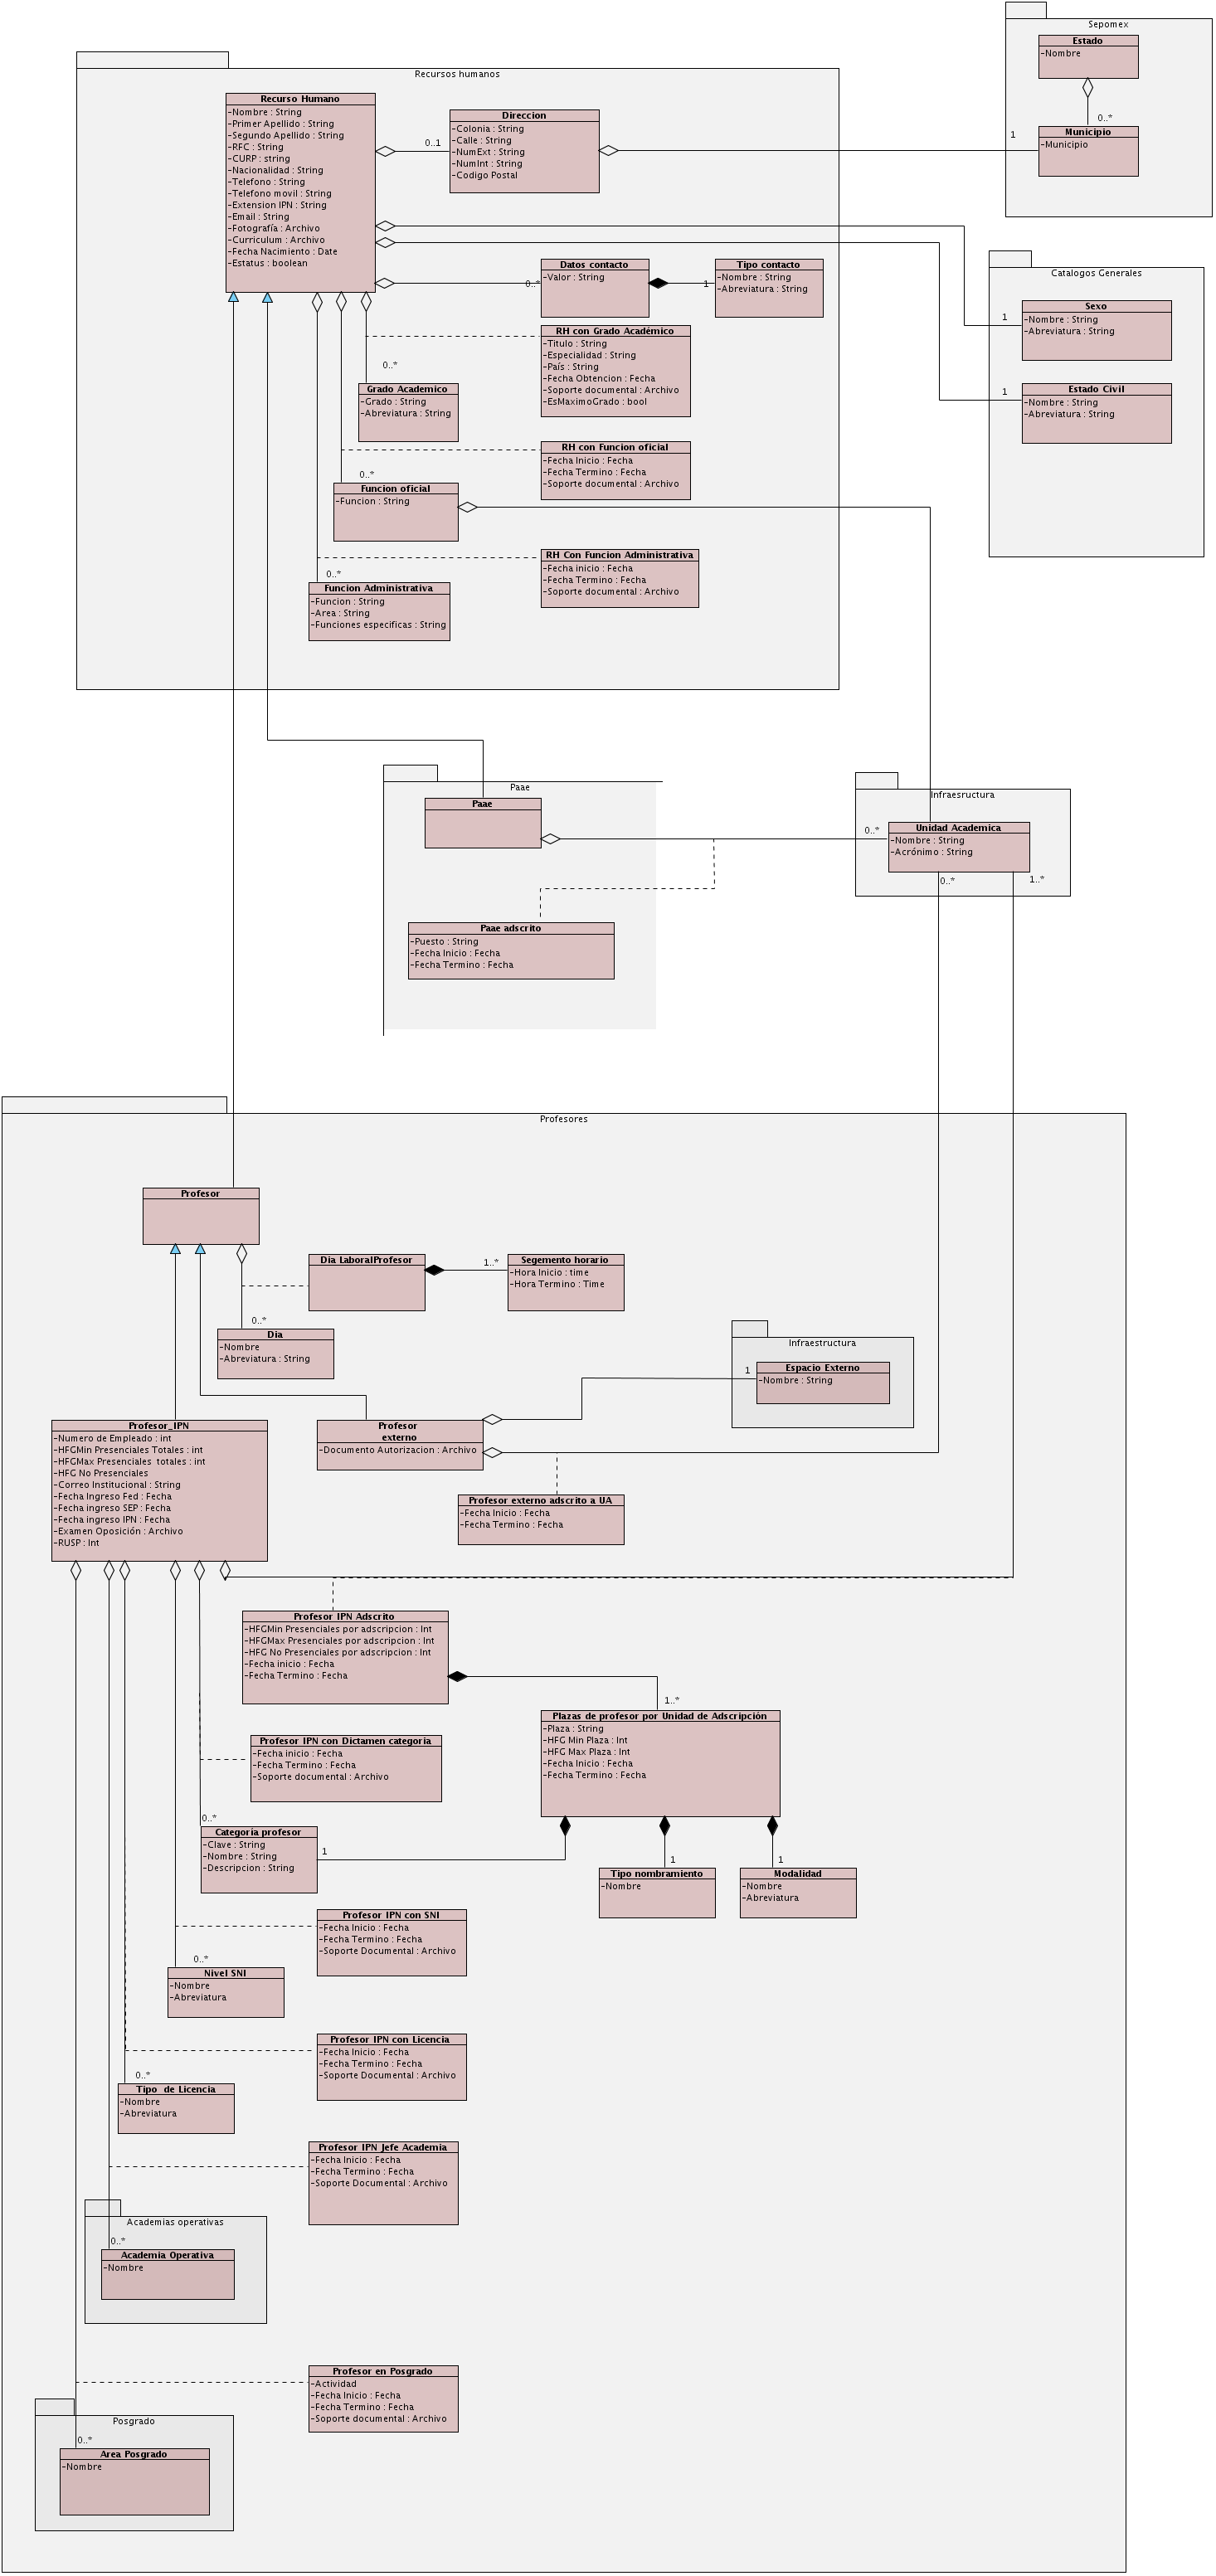
\includegraphics[width=0.5\textwidth]{negocio/images/ModeloDeInformacion_Profesores}}
		\label{fig:infoProfesores}
		\caption{Modelo de Información de Profesores}
	\end{center}
\end{figure}

%===================================Catálogos

%-------------------------------------Funcion Oficial
\begin{cdtEntidad}{FuncionOficial}{Función Oficial}
	\brAttr{funcion}{Función}{Frase}{Indica el nombre de un cargo que se encuentra dentro del siguiente catálogo:\begin{Citemize}
			\item Director
			\item Subdirector Académico
			\item Jefe de la SEPI
			\item Subdirector de Servicios Educativos e Integración Social
			\item Subdirector Administrativo
			\item Jefe de la Unidad de Informática
			\item Maestro decano
	\end{Citemize}}{\datRequerido}
	
	\brAttr{descripcion}{Descripción}{Frase}{Es una descripción corta de una función oficial en específico.}{\datRequerido}
	
	\cdtEntityRelSection
	
	\brRel{\brRelAgregation}{\refElem{UnidadAcademica}}{Una \refElem{UnidadAcademica} define al personal que ocupará una \refElem{FuncionOficial} para uno o más periodos.}
\end{cdtEntidad}



%----------------------------------Función administrativa
\begin{cdtEntidad}{RHFuncionAdministrativa}{Recurso Humando con Función Administrativa}

	\brAttr{funcionesEspecificas}{Funciones Específicas}{Frase}{Indica el nombre de un puesto dentro de una Unidad Académica que no se encuentra dentro del catálogo de Funciones Oficiales, cambiando su nombre y sus actividades dependiendo de las necesidades de una Unidad en particular.}{\datRequerido}
	
	\brAttr{area}{Área}{Frase}{Indica el nombre del área al que la función administrativa se encuentra adscrita. Por ejemplo: El Jefe de Departamento de Gestión Escolar pertenece al Área de Gestión Escolar.}{\datRequerido}
	
	\cdtEntityRelSection
	
	\brRel{\brRelAgregation}{\refElem{RecursoHumano}}{Un \refElem{RecursoHumano} del Instituto puede llegar a ocupar una \refElem{FuncionAdministrativa}, la cual es creada de acuerdo a las necesidades particulares de cada \refElem{UnidadAcademica}.}
	
\end{cdtEntidad}

%-----------------------------------Municipio
\begin{cdtEntidad}{Municipio}{Municipio}
	%=====Atributos
	
	\brAttr{nombreMunicipio}{Nombre del Municipio}{Frase}{Indica el nombre de un municipio de un Estado.}{\datRequerido}
	
	%======Relaciones
	
	\cdtEntityRelSection
	
	\brRel{\brRelAgregation}{\refElem{Direccion}}{Una \refElem{Direccion} se encuentra dentro de los límites de un \refElem{Municipio}.}
	
	\brRel{\brRelAgregation}{\refElem{Estado}}{Un \refElem{Municipio} se encuentra dentro de los límites de un \refElem{Estado}}
\end{cdtEntidad}

%----------------------------------Estado

\begin{cdtEntidad}{Estado}{Estado}
	%=======Atributos
	
	\brAttr{nombreEstado}{Nombre del Estado}{Frase}{Indica el nombre de un estado de la República Mexicana.}{\datRequerido}
	
	%=========Relaciones
	
	\cdtEntityRelSection
	
	\brRel{\brRelAgregation}{\refElem{Municipio}}{Un \refElem{Municipio} se encuentra dentro de los límites de un \refElem{Estado}}
\end{cdtEntidad}



%----------------------------------Sexo
\begin{cdtEntidad}{Sexo}{Sexo}
	%====Atributos
	
	\brAttr{nombre}{Nombre}{Palabra}{Indica el nombre de la condición orgánica que distingue a los machos de las hembras.\begin{Citemize}
			\item Masculino
			\item Femenino
	\end{Citemize}}{\datRequerido}
	
	\brAttr{abreviatura}{Abreviatura}{Caracter}{Indica la convención ortográfica que se utilizará para representar cada uno de los sexos.\begin{Citemize}
			\item Masculino \flechaDerecha M
			\item Femenino \flechaDerecha F
	\end{Citemize}}{\datRequerido}
	
	
	%= Relaciones
	\cdtEntityRelSection
	\brRel{\brRelAgregation}{\refElem{RecursoHumano}}{Un \refElem{RecursoHumano} tiene un \refElem{Sexo} pudiendo ser:
		\begin{Citemize}
			\item Masculino
			\item Femenino
	\end{Citemize}}
	
\end{cdtEntidad}


%--------------------------------------Estado Civil
\begin{cdtEntidad}{EstadoCivil}{Estado Civil}
	
	%======Atributos
	\brAttr{nombre}{Nombre}{Frase}{Indica la situación de un Recurso Humano determinada por sus relaciones de familia, provenientes del matrimonio o del parentesco, que establece ciertos derechos y deberes.\begin{Citemize}
			\item Soltero(a)
			\item Casado(a)
			\item Divorciado(a)
			\item Viudo(a) 
	\end{Citemize}}{\datRequerido}
	
	\brAttr{abreviatura}{Abreviatura}{Palabra}{Indica la convención ortográfica que se utilizará para representar cada uno de los Estados Civiles de un Recurso Humano.\begin{Citemize}
			\item Soltero(a) \flechaDerecha S
			\item Casado(a) \flechaDerecha C
			\item Divorciado(a) \flechaDerecha D
			\item Viudo(a) \flechaDerecha V
	\end{Citemize}}{\datRequerido}
	
	%========Relaciones
	\cdtEntityRelSection
	\brRel{\brRelAgregation}{\refElem{RecursoHumano}}{Un \refElem{RecursoHumano} tiene un \refElem{EstadoCivil} pudiendo ser:
		\begin{Citemize}
			\item Soltero(a)
			\item Casado(a)
			\item Divorciado(a)
			\item Viudo(a)
	\end{Citemize}}
\end{cdtEntidad}

%-----------------------------Grado Académico
\begin{cdtEntidad}{GradoAcademico}{Grado Académico}
	%=====Atributos
	
	\brAttr{grado}{Grado}{Palabra}{Describe el nombre de una distinción adquirida por una persona en una Institución Educativa de Nivel Superior y de Posgrado.\begin{Citemize}
			\item Licenciatura
			\item Maestría
			\item Doctorado
	\end{Citemize}}{\datRequerido}
	
	\brAttr{abreviatura}{Abreviatura}{Palabra}{Indica la convención ortográfica que se utilizará para representar cada uno de los Grados Académicos.\begin{Citemize}
			\item Licenciatura \flechaDerecha Lic.
			\item Maestría \flechaDerecha M. en
			\item Doctorado \flechaDerecha Dr(a). 
	\end{Citemize}}{\datRequerido}
	
	%=====Relaciones
	
	\cdtEntityRelSection
	
	\brRel{\brRelAgregation}{\refElem{GradoAcademico}}{Un \refElem{RecursoHumano} del Instituto ha conseguido varios o al menos un \refElem{GradoAcademico} a lo largo de su carrera académica.}
\end{cdtEntidad}

%----------------------------------------Tipo de Contacto

\begin{cdtEntidad}{TipoContacto}{Tipo de Contacto}
	%=======Atributos
	
	\brAttr{nombre}{Nombre}{Frase}{Indica el valor adquirido de un tipo de contacto pudiendo ser:\begin{Citemize}
			\item Email
			\item Teléfono de domicilio
			\item Teléfono móvil
	\end{Citemize}}{\datRequerido}
	
	\brAttr{abreviatura}{Abreviatura}{Palabra}{Indica la convención ortográfica que se utilizará para representar cada uno de los tipos de contacto existentes.\begin{Citemize}
			\item Email \flechaDerecha Em
			\item Teléfono de domicilio \flechaDerecha TD
			\item Teléfono móvil \flechaDerecha TM
	\end{Citemize}}{\datRequerido}
	
	%====Relaciones
	
	\cdtEntityRelSection
	
	\brRel{\brRelAgregation}{\refElem{DatoContacto}}{Un \refElem{DatoContaco} es un \refElem{TipoContacto}}
\end{cdtEntidad}

%-----------------------------------------Dia
\begin{cdtEntidad}{Dia}{Día}
	\brAttr{nombre}{Nombre}{Palabra}{Indica un valor el cual representa uno de los días de la semana, puediendo ser:
		\begin{Citemize}
			\item Lunes
			\item Martes
			\item Miércoles
			\item Jueves
			\item Viernes
			\item Sábado
			\item Domingo
	\end{Citemize}}{\datRequerido}
	\brAttr{abreviatura}{Abreviatura}{Palabra}{Indica la convención ortográfica que se utilizará para representar cada uno de los dias de la semana:
		\begin{Citemize}
			\item Lunes \flechaDerecha L
			\item Martes \flechaDerecha M
			\item Miércoles \flechaDerecha Mi
			\item Jueves \flechaDerecha J
			\item Viernes \flechaDerecha V
			\item Sábado \flechaDerecha S
			\item Domingo \flechaDerecha D
	\end{Citemize}}{\datRequerido}
	
	\cdtEntityRelSection
	
	\brRel{\brRelAgregation}{\refElem{Dia}}{Un \refElem{Profesor} realiza sus actividades de docente en uno o varios \refElem{Dia}s de la semana.}
\end{cdtEntidad}

%----------------------------------Nivel de SNI
\begin{cdtEntidad}{NivelSNI}{Nivel en el SNI}
	
	\brAttr{nombre}{Nombre}{Palabra}{Representa uno de los múltiples niveles del Sistema Nacional de Investigadores pudiendo ser:
	\begin{Citemize}
		\item Candidato
		\item Nivel I 
		\item Nivel II 
		\item Nivel III 
		\item Emérito
	\end{Citemize}}{\datRequerido}

	\brAttr{abreviatura}{Abreviatura}{Palabra}{Indica la convención ortográfica que se utilizará para representar cada uno de los niveles de SNI.\begin{Citemize}
			\item Candidato \flechaDerecha C
			\item Nivel I \flechaDerecha SNI1
			\item Nivel II \flechaDerecha SNI2
			\item Nivel III \flechaDerecha SN3
			\item Emérito \flechaDerecha E
	\end{Citemize}}{\datRequerido}

	\cdtEntityRelSection
	
	\brRel{\brRelAgregation}{\refElem{ProfesorIPN}}{Un \refElem{ProfesorIPN} puede pertenecer al SNI y adquirir un \refElem{NivelSNI}}. 
\end{cdtEntidad}

%----------------------------------Licencia
\begin{cdtEntidad}{Licencia}{Licencia}
	\brAttr{nombre}{Nombre}{Frase}{Representa el nombre de un tipo de licencia adquirible por los Profesores del Instituto pudiendo ser:
	\begin{Citemize}
		\item Licencia Con Goce de Sueldo
		\item Licencia Sin Goce de Sueldo
\end{Citemize}.}{\datRequerido}

	\brAttr{abreviatura}{Abreviatura}{Palabra}{Indica la convención ortográfica que se utilizará para representar cada una de las Licencias:\begin{Citemize}
			\item Licencia Con Goce de Sueldo \flechaDerecha LCGS
			\item Licencia Sin Goce de Sueldo \flechaDerecha LSGS
	\end{Citemize}}{\datRequerido}

	\cdtEntityRelSection
	
	\brRel{\brRelAgregation}{\refElem{ProfesorIPN}}{Un \refElem{ProfesorIPN} solicita a lo largo de su estancia en el Instituto, \refElem{Licencia} con goce de sueldo o sin goce de sueldo.}
\end{cdtEntidad}
%------------------------------------ Modalidad
\begin{cdtEntidad}{Modalidad}{Modalidad}
	\brAttr{nombre}{Nombre}{Frase}{Representa el nombre de las distintas modalidades en las que un Profesor, puede impartir clases siendo actualmente:
		\begin{Citemize}
			\item Escolarizada
			\item No Escolarizada
			\item Mixta
	\end{Citemize}, existiendo la restricción de que un Profesor de modalidad no escolarizada, no puede impartir clases en la modalidad escolarizada.}{\datRequerido}

	\brAttr{abreviatura}{Abreviatura}{Palabra}{Indica la convención ortográfica que se utilizará para representar cada una de las distintas modalidades que ofrece el Instituto:\begin{Citemize}
			\item Escolarizada \flechaDerecha ESC
			\item No Escolarizada \flechaDerecha NESC
			\item Mixta \flechaDerecha M
	\end{Citemize}}{\datRequerido}

	\cdtEntityRelSection
	
	\brRel{\brRelAgregation}{\refElem{}}{Una \refElem{} está asociada a una \refElem{Modalidad} que describe la forma en que el \refElem{ProfesorIPN} impartirá sus clases.}
\end{cdtEntidad}
%---------------------------------------------------Nombramiento
\begin{cdtEntidad}{TipodeNombramiento}{Tipo de Nombramiento}
	\brAttr{nombre}{Nombre}{Frase}{Representa el tipo }{\datRequerido}
	
	\cdtEntityRelSection
	
	\brRel{\brRelAgregation}{\refElem{}}{A una \refElem{} le corresponde un \refElem{TipodeNombramiento}}
\end{cdtEntidad}

%----------------------------------------------Categoría Plaza
\begin{cdtEntidad}{CategoriaPlaza}{Categoría de Plaza}
	\brAttr{clave}{Clave}{Palabra}{Representa un conjunto de digitos alfanumericos únicos que tienen asociada un categoría que un Profesor  adquiere por cada una de sus plazas y/o por su asosiación con el Instituto.Para conocer más acerca de estas categorías consultar el Anexo \ref{tal}. }{\datRequerido}
	
	\brAttr{nombre}{Nombre}{Frase}{Representa el nombre que una Categoría adquiere y que ayuda a determinar las horas que el Profesor debe cubrir frente a grupo para obtener su  \refElem{tCargaReglamentaria}}{\datRequerido}
	
	\cdtEntityRelSection
	\brRel{\brRelAgregation}{\refElem{ProfesorIPN}}{Un \refElem{ProfesorIPN} adquiere una \refElem{CategoriaPlaza} en el Instituto.}
	
	\brRel{\brRelAgregation}{\refElem{}}{Una \refElem{} está asoaciada a una \refElem{CategoriaPlaza}.}
\end{cdtEntidad}

%------------------------------------------Entidades que componen a otras entidades
%---------------------------------------Dirección
\begin{cdtEntidad}{Direccion}{Dirección}
	
	%=========Atributos
	\brAttr{codigoPostal}{Código Postal}{Frase}{Esquema que se asigna a distintas zonas o lugares de un país.}{\datRequerido}
	
	\brAttr{colonia}{Colonia}{Frase}{Indica el nombre de la colonia en que se encuentra una calle.}{\datRequerido}
	
	\brAttr{calle}{Calle}{Frase}{Indica el nombre de una calle en la que se encuentra un domicilio.}{\datRequerido}
	
	\brAttr{numExt}{Número Exterior}{Palabra}{Indica el número exterior que le fue asignado a un domicilio.}{\datRequerido}
	
	\brAttr{numInt}{Número Interior}{Frase}{Indica el número interior dentro de un domicilio.}{\datOpcional}
	%===================Relaciones
	\cdtEntityRelSection
	
	\brRel{\brRelComposition}{\refElem{RecursoHumano}}{Un \refElem{RecursoHumano} tiene una \refElem{Direccion} en la cual vive o recibe sus comprobantes de pago.}
	
	\brRel{\brRelAgregation}{\refElem{Municipio}}{Una \refElem{Direccion} se encuentra dentro de un \refElem{Municipio}}
\end{cdtEntidad}

%---------------------------------------Datos de Contacto
\begin{cdtEntidad}{DatoContacto}{Dato de Contacto}
	%=======Atributos
	\brAttr{valor}{Valor}{Palabra}{Es el valor adquirido por un dato de contacto.}{\datRequerido}
	
	\brAttr{tipoContacto}{Tipo de Contacto}{\refElem{TipoContacto}}{Indica qué tipo de contacto es el dato agregado.}{\datRequerido}
	%======Relaciones
	\cdtEntityRelSection
	\brRel{\brRelComposition}{\refElem{DatoContacto}}{Un \refElem{RecursoHumano} tiene uno o varios \refElem{DatoContacto} con el que es posible localizarlo.}
	
	\brRel{\brRelAgregation}{\refElem{TipoContacto}}{Un \refElem{DatoContaco} es un \refElem{TipoContacto}}
\end{cdtEntidad}

%----------------------

\begin{cdtEntidad}{UnidadAcademica}{Unidad Académica}
	\brAttr{nombre}{Nombre}{Frase}{Reppresenta el nombre con el que se conoce a unidad académica que pertenece al Instituto.}{\datRequerido}
	\brAttr{acronimo}{Acrónimo}{Palabra}{Indica la convención ortográfica que se utilizará para representar las siglas con las cuales se conoce a una Unidad Académica del Instituto. Por Ejemplo:\begin{Citemize}
			\item Escuela Superior de Cómputo \flechaDerecha ESCOM
			\item Escuela Superior de Turismo \flechaDerecha EST
	\end{Citemize}}{\datRequerido}
	
	%----Atributos
	
	\cdtEntityRelSection
	
	\brRel{\brRelAgregation}{\refElem{FuncionOficial}}{Una \refElem{UnidadAcademica} define al personal que ocupará una \refElem{FuncionOficial} para uno o más periodos.}
	
	\brRel{\brRelAgregation}{\refElem{PAAE}}{Un \refElem{PAAE} se encuentra adscrito a una o muchas unidades académicas del Instituto donde cumple funciones.}
	
	\brRel{\brRelAgregation}{\refElem{ProfesorIPN}}{Un \refElem{ProfesorIPN} se encuentra adscrito a una o varias \refElem{UnidadAcademica}.}
	
	\brRel{\brRelAgregation}{\refElem{ProfesorExterno}}{Un \refElem{ProfesorExterno} se encuentra adscrito a una o varias \refElem{UnidadAcademica}.}
	
\end{cdtEntidad}

%-------------------------------Academia Operativa
\begin{cdtEntidad}{AcademiaOperativa}{Academia Operativa}
	\brAttr{nombre}{Nombre}{Frase}{Representa a una Academia que se encuentra operando o realizando sus actividades con base en el Reglamento de Academias.}{\datRequerido}
	
	\cdtEntityRelSection
	
	\brRel{\brRelAgregation}{\refElem{ProfesorIPN}}{Un \refElem{ProfesorIPN} pertenece a una o varias \refElem{AcademiaOperativa} dentro de una \refElem{UnidadAcademica}.}
\end{cdtEntidad}


%-------------------------Área de Posgrado
\begin{cdtEntidad}{AreadePosgrado}{Área de Posgrado}
	\brAttr{nombre}{Nombre}{Frase}{Representa a un área de posgrado que se encuentra de una Unidad Académica.}{\datRequerido}
	
	\cdtEntityRelSection
	
	\brRel{\brRelAgregation}{\refElem{ProfesorIPN}}{Un \refElem{ProfesorIPN} pertenece a una o varias \refElem{AreaPosgrado}\footnote{SEPI} de una \refElem{UnidadAcademica}.}
\end{cdtEntidad}




%----------------------------------Recurso Humano--------------------------------------
\begin{cdtEntidad}{RecursoHumano}{Recurso Humano}
	\brAttr{nombre}{Nombre}{Frase}{Representa la palabra o conjunto de palabras con las que se designan y se distinguen a una Persona que labora en el Instituto.}{\datRequerido}
	
	\brAttr{primerApellido}{Primer apellido}{Frase}{Representa la palabra o conjunto de palabras que sigue al nombre de pila de una persona y que se transmite de padres a hijos.}{\datRequerido}
	
	\brAttr{segundoApellido}{Segundo apellido}{Frase}{Representa la palabra o conjunto de palabras que sigue al primer apellido de una persona y que se transmite de padres a hijos.}{\datOpcional}
	
	\brAttr{RFC}{RFC}{Palabra}{Representa la clave alfanúmerica compuesta de 13 caracteres que permite cumplir con las obligaciones que la ley establece para el pago de impuestos. En el Instituto es un mecanismo que ayuda a identificar a una persona que labora o apoya en las actividades académicas y administrativas. }{\datRequerido}
	
	\brAttr{CURP}{CURP}{Palabra}{Representa la clave alfanúmerica compuesta de 18 caracteres que permite identificar a un ciudadano residente de México. En el Instituto es otro de los mecanismos que ayudan a identificar a una persona que labora o apoya en las actividades académicas y administrativas.}{\datRequerido}
	
	\brAttr{nacionalidad}{Nacionalidad}{Frase}{Representa la condición que reconoce a una persona la pertenencia a un estado o nación, ya sea por nacimiento o que la persona haya realizado el proceso de naturalización.}{\datOpcional}
	
	\brAttr{telefono}{Teléfono}{Frase}{Representa una clave numérica que que permite conocer el número teléfonico de una persona que labora en el Instituto.}{\datOpcional}
	
	\brAttr{telefonoMovil}{Teléfono Móvil}{Frase}{Representa una clave numérica que permite conocer el número teléfonico de un dispositivo móvil de una persona que labora en el Instituto.}{\datOpcional}
	
	\brAttr{extensionIPN}{Extensión en el IPN}{Frase}{Representa una clave numérica que contiene el número  con el que es posible localizar a una persona que labora dentro de la línea privada del Instituto.}{\datOpcional}
	
	\brAttr{email}{Email}{Frase}{Representa el correo electrónico de una persona que labora en el Instituto. \refElem{RecursoHumano}.}{\datOpcional}
	
	\brAttr{fotografia}{Fotografía}{Archivo}{Es un archivo en formato JPG o PNG que contiene una imagén de la persona que labora en el Instituto.}{\datOpcional}
	
	\brAttr{curriculum}{Currículum}{Archivo}{Es un archivo que contiene los logros académicos obtenidos por la persona tanto fuera como dentro del Instituto Politécnico Nacional.}{\datOpcional}
	
	\brAttr{fechaNacimiento}{Fecha de Nacimiento}{Fecha}{Representa el conjunto de valores de día, mes y año que contiene el Acta de Nacimiento del Recurso Humano.}{\datRequerido}
	
	\brAttr{estatus}{Estatus}{Booleano}{Indica si un recurso humano del Instituto se encuentra: \begin{Citemize}
			\item Activo \flechaDerecha Indica que el Recurso Humano se encuentra realizando actividades académicas y/o administrativas,.
			\item Inactivo \flechaDerecha Indica que el Recuro Humano no se encuentra realizando actividades académicas y/o administrativas.
	\end{Citemize}}{\datOpcional}
	
	\cdtEntityRelSection
	
	\brRel{\brRelComposition}{\refElem{Direccion}}{Un \refElem{RecursoHumano} tiene una \refElem{Direccion} en la cual vive o recibe sus comprobantes de pago.}
	
	\brRel{\brRelAgregation}{\refElem{Sexo}}{Un \refElem{RecursoHumano} tiene un \refElem{Sexo} pudiendo ser:
		\begin{Citemize}
			\item Masculino
			\item Femenino
	\end{Citemize}}
	
	\brRel{\brRelAgregation}{\refElem{EstadoCivil}}{Un \refElem{RecursoHumano} tiene un \refElem{EstadoCivil} pudiendo ser:
		\begin{Citemize}
			\item Soltero(a)
			\item Casado(a)
			\item Divorciado(a)
			\item Viudo(a)
	\end{Citemize}}
	
	\brRel{\brRelComposition}{\refElem{DatoContacto}}{Un \refElem{RecursoHumano} tiene uno o varios \refElem{DatoContacto} con el que es posible localizarlo.}
	
	\brRel{\brRelAgregation}{\refElem{GradoAcademico}}{Un \refElem{RecursoHumano} del Instituto ha conseguido varios o al menos un \refElem{GradoAcademico} a lo largo de su carrera académica.}
	
	\brRel{\brRelAgregation}{\refElem{FuncionOficial}}{Un \refElem{RecursoHumano} del Instituto puede llegar a ocupar una \refElem{FuncionOficial} en una \refElem{UnidadAcademica}.}
	
	\brRel{\brRelAgregation}{\refElem{FuncionAdministrativa}}{Un \refElem{RecursoHumano} del Instituto puede llegar a ocupar una \refElem{FuncionAdministrativa}, la cual es creada de acuerdo a las necesidades particulares de cada \refElem{UnidadAcademica}. Pueden ser:
		\begin{Citemize}
			\item Jefe(a) del Departamento de Gestión Escolar.
			\item Jefe(a) del Departamento de Servicios Educativos.
			\item Jefe(a) del Departamento de Extensión y Apoyos Educativas
	\end{Citemize}}
	
	\brRel{\brRelGeneralization}{\refElem{Profesor}}{Un \refElem{RecursoHumano}  es un \refElem{Profesor} o docente que imparte clases en una o varias unidades académicas\footnote{ver \refElem{UnidadAcademica}}.}
	
	\brRel{\brRelGeneralization}{\refElem{PAAE}}{Un \refElem{RecursoHumano} es un \refElem{PAAE}}
	
\end{cdtEntidad}


%---------------------------------------RHGrado Académico--------------------------------------------%
\begin{cdtEntidad}{RHGradoAcademico}{Recurso Humano con Grado Académico}
	%====Atributos
	\brAttr{titulo}{Titulo}{Frase}{Indica el nombre de un grado  específico adquirido por un \refElem{RecursoHumano}. Por ejemplo:\begin{Citemize}
			\item Licenciado en Ingeniería en Sistemas Computacionales,
			\item Maestro en Ciencias de la Computación
	\end{Citemize}}{\datRequerido}
	
	\brAttr{especialidad}{Especialidad}{Frase}{Indica el nombre de una especialidad , si la tuviese, del titulo adquirido.}{\datOpcional}
	
	\brAttr{pais}{País}{Frase}{Indica el nombre de la comunidad social con una organización política común y un territorio y órganos de gobierno propios que es independiente políticamente de otras comunidades donde el Recurso Humano adquirió el \refElem{GradoAcademico}.}{\datRequerido}
	
	\brAttr{fechaObtencion}{Fecha de Obtención}{Fecha}{Representa el conjunto de valores de día, mes y año que contiene el documento donde se avalá que la persona adquirió el grado academico.}{\datRequerido}
	
	\brAttr{soporteDocumental}{Soporte Documental}{Archivo}{Es un archivo o conjunto de archivos que contienen las imágenes de los documentos que validan que el \refElem{RecursoHumano} adquirió el \refElem{GradoAcademico}.}{\datOpcional}
	
	\brAttr{esMaximoGrado}{Máximo Grado}{Booleano}{Indica si el grado adquirido es el máximo obtenido por el \refElem{RecursoHumano}}{\datRequerido}
\end{cdtEntidad}

%--------------------Funcion Oficial en Unidad Académica
\begin{cdtEntidad}{FuncionOficialenUnidadAcademica}{Función Oficial en Unidad Académica}
	
	\brAttr{unidad}{Unidad}{\refElem{UnidadAcademica}}{Indica la Unidad Académica a la que pertenece una Función Oficial.}{\datRequerido}
	
	\brAttr{funcion}{Función}{\refElem{FuncionOficial}}{Indica la función oficial que una unidad académca tiene.}{\datRequerido}
	
	\cdtEntityRelSection
	
	\brRel{\brRelAgregation}{\refElem{RecursoHumano}}{Un \refElem{RecursoHumano} del Instituto puede llegar a ocupar una \refElem{FuncionOficial} en una \refElem{UnidadAcademica}.}
\end{cdtEntidad}

%------------Recurso Humano con Función Oficial
\begin{cdtEntidad}{RHFuncionOficial}{Recurso Humano con Función Oficial}
	
	\brAttr{fechaInicio}{Fecha de Inicio}{Fecha}{Representa el conjunto de valores de día, mes y año que están contenidas en el documento que avala que un recurso humano adquirió una función oficial.}{\datRequerido}
	
	\brAttr{fechaTermino}{Fecha de Término}{Fecha}{Representa el conjunto de valores de día, mes y año que están contenidas en el documento que avala la fecha en que el recurso humano concluye su función oficial.}{\datRequerido}
	
	\brAttr{soporteDocumental}{Soporte Documental}{Archivo}{Es el archivo o conjunto de archivos, en cualquier formato digital, que avala la adquisición de la función oficial.}{\datRequerido}
\end{cdtEntidad}

%------------------------------------------------RHFuncionAdministrativa

\begin{cdtEntidad}{RHFuncionAdministrativa}{Recurso Humano con Función Administrativa}
	\brAttr{fechaInicio}{Fecha de Inicio}{Fecha}{Representa el conjunto de valores de día, mes y año que están contenidas en el documento que avalá que un Recurso Humano adquirió una Función Administrativa.}{\datRequerido}
	
	\brAttr{fechaTermino}{Fecha de Término}{Fecha}{Representa el conjunto de valores de día, mes y año que están contenidas en el documento que avala la fecha en que el Recurso Humano concluye su Función Administrativa.}{\datRequerido}
	
	\brAttr{soporteDocumental}{Soporte Documental}{Archivo}{Es el archivo o conjunto de archivos, en cualquier formato digital, que avala la adquisición de la función admiministrativa.}{\datRequerido}
\end{cdtEntidad}

%----------------------------------PAAE
\begin{cdtEntidad}{PAAE}{Personal de Apoyo y Asistenica a la Educación}
	%----------Relaciones
	\cdtEntityRelSection
	
	\brRel{\brRelGeneralization}{\refElem{RecursoHumano}}{Un \refElem{RecursoHumano} es un \refElem{PAAE}}
	
	\brRel{\brRelAgregation}{\refElem{UnidadAcademica}}{Un \refElem{PAAE} se encuentra adscrito a una o muchas unidades académicas del Instituto donde realiza las actividades correspondientes a este rol.}
\end{cdtEntidad}


%----------------PAAE Adscrito
\begin{cdtEntidad}{PAAEAdscrito}{PAAE Adscrito}
	\brAttr{puesto}{Puesto}{Frase}{Indica el nombre del puesto que el PAAE adquirió en una Unidad Académica.}{\datRequerido}
	
	\brAttr{fechaInicio}{Fecha de Inicio}{Fecha}{Representa el conjunto de valores de día, mes y año que describen la fecha en que el PAAE adquirió el puesto dentro de una Unidad Académica y en la cual sus funciones son aplicables.}{\datRequerido}
	
	\brAttr{fechaTermino}{Fecha de Término}{Fecha}{Representa el conjunto de valores de día, mes y año que describen la fecha en que el PAAE concluye sus funciones dentro de una Unidad Académica.}{\datRequerido}
\end{cdtEntidad}



%----------------------------------Profesor
\begin{cdtEntidad}{Profesor}{Profesor}
	\cdtEntityRelSection
	
	\brRel{\brRelGeneralization}{\refElem{RecursoHumano}}{Un \refElem{RecursoHumano}  es un \refElem{Profesor} o docente que imparte clases en una o varias unidades académicas.}
	
	\brRel{\brRelGeneralization}{\refElem{ProfesorIPN}}{Un \refElem{ProfesorIPN} es un \refElem{Profesor} del Instituo.}
	
	\brRel{\brRelGeneralization}{\refElem{ProfesorExterno}}{Un\refElem{ProfesorExterno} es un \refElem{Profesor} que apoya en las labores académicas y docentes del Instituto, sin tener una relación estrictamente laboral.}
	
	\brRel{\brRelAgregation}{\refElem{Dia}}{Un \refElem{Profesor} realiza sus actividades de docente en uno o varios \refElem{Dia}s de la semana.}
	
\end{cdtEntidad}



%------------------------------------Dia Laboral
\begin{cdtEntidad}{DiaLaboral}{Día Laboral}
	\cdtEntityRelSection
	
	\brRel{\brRelComposition}{\refElem{SegmentoHorario}}{Un \refElem{Profesor} dentro de un \refElem{DiaLaboral} tiene \refElem{SegmentoHorario} en los que realiza sus actividades de docente.}
\end{cdtEntidad}

%------------------------------------Segmento de Horario
\begin{cdtEntidad}{SegmentoHorario}{Segmento de Horario}
	\brAttr{horaInicio}{Hora de Inicio}{Horas}{Representa el conjunto de valores de hora y minutos que describen la hora en que el Profesor inicia un segmento de horario de un día laboral.}{\datRequerido}
	
	\brAttr{horaFinal}{Hora Final}{Horas}{Representa el conjunto de valores de hora y minutos que describen la hora en que el Profesor concluye un segmento de horario de un día laboral}{\datRequerido}
	
	\cdtEntityRelSection
	
	\brRel{\brRelComposition}{\refElem{DiaLaboral}}{Un \refElem{Profesor} dentro de un \refElem{DiaLaboral} tiene \refElem{SegmentoHorario} en los que realiza sus actividades de docente.}
\end{cdtEntidad}

%-----------------------------------Profesor IPN

\begin{cdtEntidad}{ProfesorIPN}{Profesor del Instituto}
	\brAttr{numeroEmpleado}{Número de Empleado}{Entero}{Indica el número asignado por Capital Humano a un Profesor del Instituto cuando este fue admitido en su plantilla.}{\datRequerido}
	
	\brAttr{HFGMin}{Horas Frente a Grupo Mínimas Presenciales Totales}{Entero}{Indica el número de horas mínimas que un Profesor del Instituto debe cubrir impartiendo clase.}{\datRequerido}
	
	\brAttr{HFGMax}{Horas Frente a Grupo Máximas Presenciales Totales}{Entero}{Indica el número de horas máximas que un Profesor del Instituto debe cubrir impartiendo clase.}{\datRequerido}
	
	\brAttr{HGFnoPresenciales}{Horas Frente a Grupo No Presenciales}{Entero}{}{\datRequerido}
	
	\brAttr{correoInstitucional}{Correo Electrónico Institucional}{Frase}{Indica el correo electrónico que le fue asignado a un \refElem{ProfesorIPN}.}{\datOpcional}
	
	\brAttr{fechaIngresoFed}{Fecha de Ingreso al Gobierno Federal}{Fecha}{Indica la fecha en el que Profesor se incorporó al Gobierno Federal.}{\datRequerido}
	
	\brAttr{fechaIngresoSEP}{Fecha de Ingreso a la SEP}{Fecha}{Indica la fecha en el que Profesor se incorporó a la Secretaría de Educación Pública.}{\datRequerido}
	
	\brAttr{fechaIngresoIPN}{Fecha de Ingreso al Instituto}{Fecha}{Indica la fecha en el que Profesor se incorporó al Instituto Politécnico Nacional.}{\datRequerido}
	
	\brAttr{examenOposicion}{Examen de Oposición}{Archivo}{Archivo que contiene el examen de oposición presentado por el Profesor que avala su incorporación a un Academía de una Unidad Académica.}{\datRequerido}
	
	\brAttr{RUSP}{RUSP}{Entero}{Indica el número del  Registro de Servidores Públicos del Gobierno Federal asignado al Profesor.}{\datOpcional}
	
	\cdtEntityRelSection
	
	\brRel{\brRelGeneralization}{\refElem{Profesor}}{Un \refElem{ProfesorIPN} es un \refElem{Profesor} del Instituo.}
	
	\brRel{\brRelAgregation}{\refElem{UnidadAcademica}}{Un \refElem{ProfesorIPN} se encuentra adscrito a una o varias \refElem{UnidadAcademica}.}
	
	\brRel{\brRelAgregation}{\refElem{Categoria}}{Un \refElem{ProfesorIPN} tiene una \refElem{Categoria} de acuerdo al Tabulador de Sueldos del Personal Docente.}
	
	\brRel{\brRelAgregation}{\refElem{NivelSNI}}{Un \refElem{ProfesorIPN} puede adquirir un nivel en el Sistema Nacional de Investigadores.}
	
	\brRel{\brRelAgregation}{\refElem{Licencia}}{Un \refElem{ProseforIPN} puede solicitar una licencia de tipo:
		\begin{Citemize}
			\item Licencia con Goce de Sueldo
			\item Licencia sin Goce de Sueldo
	\end{Citemize}}
		
	\brRel{\brRelAgregation}{\refElem{AreaPosgrado}}{Un \refElem{ProfesorIPN} pertenece a una o varias \refElem{AreaPosgrado}\footnote{SEPI} de una \refElem{UnidadAcademica}.}
	
\end{cdtEntidad}

%------------------------ProfesorIPNAdscrito

\begin{cdtEntidad}{ProfesorIPNAdscrito}{Profesor del Instituto Adscrito}
	\brAttr{HGFMinPresenciales}{Horas Frente a Grupo Mínimas Presenciales por Adscripción}{Entero}{Indica el número de horas mínimas que el Profesor debe cubrir impartiendo clases en una Unidad Académica}{\datRequerido}
	
	\brAttr{HGFMaxPresenciales}{Horas Frente a Grupo Máximas Presenciales por Adscripción}{Entero}{Indica el número de horas máximas que el Profesor debe cubrir impartiendo clases en una Unidad Académica}{\datRequerido}
	
	\brAttr{HFGNoPresenciales}{Horas Frente a Grupo No Presenciales por Adscripción}{Entero}{}{\datRequerido}
	
	\brAttr{FechaInicio}{Fecha de Inicio}{Fecha}{Indica la fecha en que el Profesor inicia sus labores docentes en una Unidad Académica.}{\datRequerido}
	
	\brAttr{FechaTermino}{Fecha de Término}{Fecha}{Indica la fehca en que el Profesor concluye sus labores docentes una Unidad Académica.}{\datRequerido}
	
	\cdtEntityRelSection
	
	\brRel{\brRelComposition}{\refElem{PlazaPorUnidadAdscripcion}}{Un \refElem{ProfesorIPNAdscrito} tiene una o varias \refElem{PlazaPorUnidadAdscripcion} que indican el número de horas mínimas y máximas que debe cubrir en esa unidad.}
	
\end{cdtEntidad}


%--------------------------------------------PLazas del Profesor
\begin{cdtEntidad}{PlazaPorUnidadAdscripcion}{Plaza del Profesor por Unidad de Adscripción}
	\brAttr{plaza}{Plaza}{Palabra}{Indica la \refElem{tPlaza} que el Profesor está cubriendo en una Unidad Académica.}{\datRequerido}
	
	\brAttr{HFGMinPlaza}{Horas Frente a Grupo Mínimas de la Plaza}{Entero}{Indica el número mínimo de horas que un Profesor debe cubrir frente a grupo por plaza.}{\datRequerido}
	
	\brAttr{HFGMaxPlaza}{Horas Frente a Grupo Máximas de la Plaza}{Entero}{Indica el número máximo de horas que un Profesor debe cubrir frente a grupo por plaza.}{\datRequerido}
	
	\brAttr{fechaInicio}{Fecha de Inicio}{Fecha}{Indica la fecha en que la plaza comienza a tener efectos.}{\datRequerido}
	
	\brAttr{fechaTermino}{Fecha de Término}{Fecha}{Indica la fecha en que la plaza deja de tener efectos.}{\datRequerido}
	
	\cdtEntityRelSection
	
	\brRel{\brRelComposition}{\refElem{ProfesorIPNAdscrito}}{Un \refElem{ProfesorIPNAdscrito} tiene una o varias \refElem{PlazaPorUnidadAdscripcion} que indican el número de horas mínimas y máximas que debe cubrir en esa unidad.}
	
	\brRel{\brRelAgregation}{\refElem{CategoriaPlaza}}{Una \refElem{PlazaPorUnidadAdscripcion} tiene una \refElem{CategoriaPlaza}.}
	
	\brRel{\brRelAgregation}{\refElem{TipoNombramiento}}{Una \refElem{PlazaPorUnidadAdscripcion} tiene un \refElem{TipoNombramiento}}
	
	\brRel{\brRelAgregation}{\refElem{Modalidad}}{Una \refElem{PlazaPorUnidadAdscripcion} tiene una \refElem{Modalidad} pudiendo ser:
		\begin{Citemize}
			\item Escolarizada
			\item No Escolarizada
	\end{Citemize}}
\end{cdtEntidad}

%---------------------------------------------Categoria Plaza

\begin{cdtEntidad}{CategoriaPlaza}{Categoría de una Plaza}
	\brAttr{clave}{Clave}{Categoria Profesor}{Indica la clave de una de las categorias existentes.}{\datRequerido}
	
	\cdtEntityRelSection
	\brRel{\brRelAgregation}{\refElem{PlazaPorUnidadAdscripcion}}{Una \refElem{PlazaPorUnidadAdscripcion} tiene una \refElem{CategoriaPlaza}.}
\end{cdtEntidad}


%-------------Profesor Externo
\begin{cdtEntidad}{ProfesorExterno}{Profesor Externo}
	\brAttr{documentoAprobaatorio}{Documento Aprobatorio}{Archivo}{Es el archivo o conjunto de archivos que avalan que un Profesor Externo puede impartir clases para un Período.}{\datRequerido}
	
	\cdtEntityRelSection
	
	\brRel{\brRelAgregation}{\refElem{UnidadAcademica}}{Un \refElem{ProfesorExterno} se encuentra adscrito a una o varias \refElem{UnidadAcademica}.}
	
	\brRel{\brRelAgregation}{\refElem{EspacioExterno}}{Un \refElem{ProfesorExterno} se encuentra trabajando o apoyando en un \refElem{EspacioExterno} donde realiza sus actividades.}
\end{cdtEntidad}

%---------------------------Profesor Externo Adscrito a Unidad Académica
\begin{cdtEntidad}{ProfesorExternoAdscritoaUnidasAcademica}{Profesor Adscrito a Unidad Académica}
	\brAttr{fechaInicio}{Fecha de Inicio}{Fecha}{Representa el conjunto de valores de día, mes y año que describen la fecha en que un Profesor Externo iniciará sus actividades de apoyo y docencia.}{\datRequerido}
	
	\brAttr{fechaTermino}{Fecha de Término}{Fecha}{Representa el conjunto de valores de día, mes y año que describen la fecha en que un Profesor Externo concluye sus actividades de apoyo y docencia.}{\datRequerido}
\end{cdtEntidad}

%-------------------------------------Profesor Jefe de Academia
\begin{cdtEntidad}{ProfesorIPNJefedeAcademia}{Profesor del Instituto Jefe de Academia}
	\brAttr{fechaInicio}{Fecha de Inicio}{Fecha}{Representa el conjunto de valores de día, mes y año que están contenidas en el documento que avala que un recurso humano adquirió la función de presidente/jefe de Academia.}{\datRequerido}
	\brAttr{fechaTermino}{Fecha de Términio}{Fecha}{Representa el conjunto de valores de día, mes y año que están contenidas en el documento que avala la fecha en que el recurso humano concluye su período como presidente/jefe de Academia}{\datRequerido}
	\brAttr{soporteDocumental}{Soporte Documental}{Archivo}{Es el archivo o conjunto de archivos, en cualquier formato digital, que avala la adquisición de la función de presidente/jefe de academia.}{\datRequerido}
\end{cdtEntidad}

%---------------------------------------------Profesor en Área de Posgrado
\begin{cdtEntidad}{ProfesorenPosgrado}{Profesor en Posgrado}
	\brAttr{actividad}{Actividad}{Frase}{Describe las funciones y/o actividades que el Profesor realiza en el área de posgrado.}{\datRequerido}
	
	\brAttr{fechaInicio}{Fecha de Inicio}{Fecha}{Representa el conjunto de valores de día, mes y año que están contenidas en el documento que avala que un recurso humano adquirió una función o actividad a realizar en el área de Posgrado de una Unidad Académica.}{\datRequerido}
	
	\brAttr{fechaTermino}{Fecha de Término}{Fecha}{Representa el conjunto de valores de día, mes y año que están contenidas en el documento que avala la fecha en que el recurso humano concluye sus actividades o funciones en el área de Posgrado de una Unidad Académica.}{\datRequerido}
	
	\brAttr{soporteDocumental}{Soporte Documental}{Archivo}{Es el archivo o conjunto de archivos, en cualquier formato digital, que avala la adquisición de la función y/o actividades del área de psogrado de una unidad académica.}{\datRequerido}
\end{cdtEntidad}
